\chapter[Practical Hybrid Quantum-Classical Computing]{Practical Hybrid Quantum-Classical\\Computing} \label{chap:practical-hybrid-quantum-classical-computing}
This chapter is focused on the practical execution of \glspl{hqca} using the Quantum Inspire quantum computing platform and SURF's \gls{hpc} center.
% TODO: expand

\section{Quantum Inspire}
Quantum Inspire is a full-stack quantum computing platform that QuTech launched last year to make quantum systems available to the general public for exploratory research~\cite{last2020quantum}.
Users can run quantum circuits on different back-ends through the Quantum Inspire web editor or by using the Python \gls{sdk}.
The \gls{cqasm}~\cite{khammassi2018cqasm} is used for describing quantum circuits, but the popular quantum computing frameworks ProjectQ~\cite{steiger2018projectq} and Qiskit~\cite{qiskit} are also supported by the Python \gls{sdk}.
Quantum Inspire supports the execution of quantum circuits on real \glspl{qpu} and through quantum simulation.
An overview of the Quantum Inspire workflow and available device back-ends is shown in \Cref{fig:qi-workflow}.

The two available \glspl{qpu} are Starmon-5 and Spin-2 which have five and two qubits respectively.
These \glspl{qpu} suffer from noise, limited coherence time, limited qubit connectivity, and each \gls{qpu} has a specific allowed gate set.
Note that these gate sets are universal, and non-native gates are decomposed into supported gates depending on the \gls{qpu}.
Regardless of the limitations of these \glspl{qpu}, they are an essential part in research towards better quantum hardware and quantum algorithms.
\begin{figure}[ht]
    \centering
    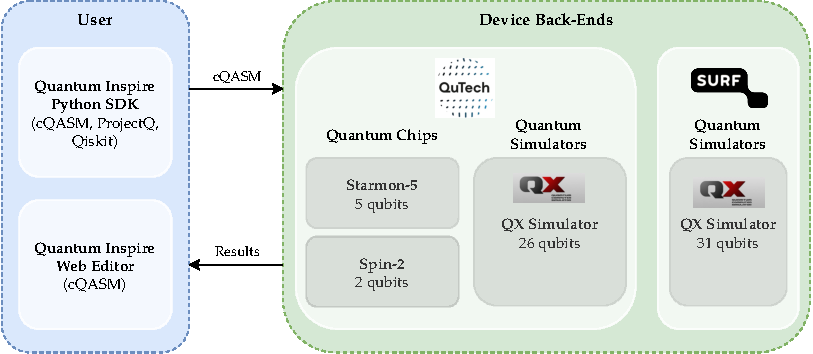
\includegraphics[width=1\linewidth]{figures/qi-workflow.pdf}
    \caption[Overview of the Quantum Inspire workflow.]{
        Overview of the Quantum Inspire workflow.
        Users can submit quantum circuits written in \gls{cqasm} using the web editor or Python \gls{sdk}.
        After the program has been run, the results are returned to the user.
        The quantum circuit can be executed on one of the \glspl{qpu} or simulated using one of the QX simulator back-ends.
        QuTech's simulator back-end supports simulations up to 26 qubits, while SURF's simulator back-end supports simulations up to 31 qubits.
    }
    \label{fig:qi-workflow}
\end{figure}

In the absence of large-scale and fault-tolerant quantum computers, quantum computer simulation is critical for developing and testing quantum algorithms.
Quantum Inspire offers two simulator back-ends which use QX~\cite{khammassi2017qx} as quantum computer simulator.
One of the simulator back-ends is hosted by QuTech on a commodity cloud-based server with 4 GB of memory, which can run simulations up to 26 qubits.
The other simulator back-end is hosted on SURF's computer cluster Lisa which consists of several hundreds of multi-core nodes.
The largest node available on Lisa has 256 GB of memory, which supports simulations up to 31 qubits.

When quantum circuits are submitted to Quantum Inspire, they are handed to a job scheduler which will attempt to schedule the job as quickly as possible when the requested resources are available.
For the \glspl{qpu} and QuTech simulator back-ends, the jobs are simply placed in a queue which are executed in first-in-first-out order.
The wait time for these back-ends ranges from seconds to minutes.
For the SURF simulator back-end, the jobs are handled by a batch system.
Because SURF's infrastructure is shared with many other users, wait times can vary from minutes to hours.
Especially large simulations which require a large amount of resources may take a long time to schedule.

\section{SURF High Performance Computing}
SURF offers an integrated ICT research infrastructure and provides services in the areas of computing, data storage, visualization, networking, and cloud.
This report is mainly interested in the computing services, and more precisely the Lisa and Cartesius cluster computers.
These cluster computers can be thought of as a network of computers (nodes).
Each node has its own \glspl{cpu}, memory, disk space, and a shared file system.
Cluster computers are often used for \acrfull{hpc}, where a large amount of resources (\glspl{cpu}, \glspl{gpu}, memory etc.) are used to solve computationally expensive problems.
Interacting with a cluster computer works different than a regular computer: instead of submitting a script or command (job) and immediately being run, cluster computers use a batch system that runs your job as soon as sufficient resources are available.
Lisa and Cartesius use the Slurm workload manager~\cite{yoo2003slurm} as job scheduler.
The specifications of the Lisa and Cartesius cluster computers are described in \Cref{table:surf-cluster-computers}.

\begin{table}[ht]
    \centering
    \begin{tabular}{ c|c|c }
        Resource & Lisa & Cartesius \\
        \hline
        \glspl{cpu} & 5304 & 47,776   \\
        Memory & 41.7 TB & 130 TB \\
        \glspl{gpu} & 216 & 132 \\
        Flop/s (64-bit floating point) & 367.9 Tflop/s & 1.843 Pflop/s  \\
        Disk space & 400 TB home & 180 TB home, 7.7 PB project + scratch \\
    \end{tabular}
    \caption[Specification of the Lisa and Cartesius cluster computers.]{
        Specification of the Lisa and Cartesius cluster computers.
        Here Flop/s refers to floating point operations per second, or the theoretical peak performance.
        Cartesius is the Dutch national supercomputer meant for large computations that require many cores, large symmetric multiprocessing nodes, large amounts of memory, a fast interconnect, large amount of disk space, or a fast I/O subsystem.
        Lisa is meant for tasks that need large computing capacities, but do not need the facilities of a real supercomputer.
    }
    \label{table:surf-cluster-computers}
\end{table}

The Lisa and Cartesius cluster computers consist of login nodes and batch nodes.
You connect to the system through the login node, which is an interactive system similar to a personal computer.
These login nodes can be used for light tasks such as writing and compiling software, writing job scripts, and preparing data.
A job script is essentially a recipe of commands that you want your job job to execute.
Through this script you can load the required modules, handle input and output data processing, define the amount of resources your job requires, and handle the running of the actual application.
The job script is submitted to the job scheduler and will be run on a batch node as soon as the requested resources are available.

\section{Hybrid Quantum-Classical Workflows}
\begin{table}[ht]
    \centering
    {\renewcommand{\arraystretch}{1.35}
        \begin{tabular}{ c|c|c|>{\centering\arraybackslash}m{4.9cm} }
            Workflow name & Classical part & Quantum part & Use case(s) \\
            \hline
            Local-Local & Local & Simulation (Local) & Small experimentation/prototyping \\
            \hline
            Local-\gls{hpc} & Local & Simulation (\gls{hpc}) & Large quantum simulations that can not be run locally \\
            \hline
            Local-\gls{qpu} & Local & \gls{qpu} & Small experimentation/exploration of hardware \\
            \hline
            \gls{hpc}-\gls{qpu} & \gls{hpc} & \gls{qpu} & Well-defined/multiple experiments, hybrid computation with expensive classical part \\
            \hline
            \gls{hpc}-\gls{hpc} & \gls{hpc} & Simulation (\gls{hpc}) & Multiple experiments, expensive classical and/or quantum part, high performance simulations \\
        \end{tabular}
    }
    \caption[Relevant hybrid quantum-classical workflows and their use cases.]{
        Relevant hybrid quantum-classical workflows and their use cases.
        In the classical part column the platform on which the classical computation runs: locally on a laptop or personal computer, or on SURF's \gls{hpc} center.
        Equivalently, the quantum part columns refers to the platform the quantum computation runs on: local simulation, \gls{qpu}, or simulation on SURF's \gls{hpc} center.
    }
    \label{table:hqca-workflows}
\end{table}
% mostly research towards HQCA's, not really practical applications/no speedups to be gained yet
% most research towards HQCA's doesnt need supercomputers - can still be useful for running multiple experiments